% Options for packages loaded elsewhere
\PassOptionsToPackage{unicode}{hyperref}
\PassOptionsToPackage{hyphens}{url}
%
\documentclass[
  ignorenonframetext,
]{beamer}
\usepackage{pgfpages}
\setbeamertemplate{caption}[numbered]
\setbeamertemplate{caption label separator}{: }
\setbeamercolor{caption name}{fg=normal text.fg}
\beamertemplatenavigationsymbolsempty
% Prevent slide breaks in the middle of a paragraph
\widowpenalties 1 10000
\raggedbottom
\setbeamertemplate{part page}{
  \centering
  \begin{beamercolorbox}[sep=16pt,center]{part title}
    \usebeamerfont{part title}\insertpart\par
  \end{beamercolorbox}
}
\setbeamertemplate{section page}{
  \centering
  \begin{beamercolorbox}[sep=12pt,center]{part title}
    \usebeamerfont{section title}\insertsection\par
  \end{beamercolorbox}
}
\setbeamertemplate{subsection page}{
  \centering
  \begin{beamercolorbox}[sep=8pt,center]{part title}
    \usebeamerfont{subsection title}\insertsubsection\par
  \end{beamercolorbox}
}
\AtBeginPart{
  \frame{\partpage}
}
\AtBeginSection{
  \ifbibliography
  \else
    \frame{\sectionpage}
  \fi
}
\AtBeginSubsection{
  \frame{\subsectionpage}
}
\usepackage{lmodern}
\usepackage{amssymb,amsmath}
\usepackage{ifxetex,ifluatex}
\ifnum 0\ifxetex 1\fi\ifluatex 1\fi=0 % if pdftex
  \usepackage[T1]{fontenc}
  \usepackage[utf8]{inputenc}
  \usepackage{textcomp} % provide euro and other symbols
\else % if luatex or xetex
  \usepackage{unicode-math}
  \defaultfontfeatures{Scale=MatchLowercase}
  \defaultfontfeatures[\rmfamily]{Ligatures=TeX,Scale=1}
\fi
% Use upquote if available, for straight quotes in verbatim environments
\IfFileExists{upquote.sty}{\usepackage{upquote}}{}
\IfFileExists{microtype.sty}{% use microtype if available
  \usepackage[]{microtype}
  \UseMicrotypeSet[protrusion]{basicmath} % disable protrusion for tt fonts
}{}
\makeatletter
\@ifundefined{KOMAClassName}{% if non-KOMA class
  \IfFileExists{parskip.sty}{%
    \usepackage{parskip}
  }{% else
    \setlength{\parindent}{0pt}
    \setlength{\parskip}{6pt plus 2pt minus 1pt}}
}{% if KOMA class
  \KOMAoptions{parskip=half}}
\makeatother
\usepackage{xcolor}
\IfFileExists{xurl.sty}{\usepackage{xurl}}{} % add URL line breaks if available
\IfFileExists{bookmark.sty}{\usepackage{bookmark}}{\usepackage{hyperref}}
\hypersetup{
  pdftitle={How to write an R package and publish it on GitHub},
  pdfauthor={Aya Mitani},
  hidelinks,
  pdfcreator={LaTeX via pandoc}}
\urlstyle{same} % disable monospaced font for URLs
\newif\ifbibliography
\usepackage{color}
\usepackage{fancyvrb}
\newcommand{\VerbBar}{|}
\newcommand{\VERB}{\Verb[commandchars=\\\{\}]}
\DefineVerbatimEnvironment{Highlighting}{Verbatim}{commandchars=\\\{\}}
% Add ',fontsize=\small' for more characters per line
\usepackage{framed}
\definecolor{shadecolor}{RGB}{248,248,248}
\newenvironment{Shaded}{\begin{snugshade}}{\end{snugshade}}
\newcommand{\AlertTok}[1]{\textcolor[rgb]{0.94,0.16,0.16}{#1}}
\newcommand{\AnnotationTok}[1]{\textcolor[rgb]{0.56,0.35,0.01}{\textbf{\textit{#1}}}}
\newcommand{\AttributeTok}[1]{\textcolor[rgb]{0.77,0.63,0.00}{#1}}
\newcommand{\BaseNTok}[1]{\textcolor[rgb]{0.00,0.00,0.81}{#1}}
\newcommand{\BuiltInTok}[1]{#1}
\newcommand{\CharTok}[1]{\textcolor[rgb]{0.31,0.60,0.02}{#1}}
\newcommand{\CommentTok}[1]{\textcolor[rgb]{0.56,0.35,0.01}{\textit{#1}}}
\newcommand{\CommentVarTok}[1]{\textcolor[rgb]{0.56,0.35,0.01}{\textbf{\textit{#1}}}}
\newcommand{\ConstantTok}[1]{\textcolor[rgb]{0.00,0.00,0.00}{#1}}
\newcommand{\ControlFlowTok}[1]{\textcolor[rgb]{0.13,0.29,0.53}{\textbf{#1}}}
\newcommand{\DataTypeTok}[1]{\textcolor[rgb]{0.13,0.29,0.53}{#1}}
\newcommand{\DecValTok}[1]{\textcolor[rgb]{0.00,0.00,0.81}{#1}}
\newcommand{\DocumentationTok}[1]{\textcolor[rgb]{0.56,0.35,0.01}{\textbf{\textit{#1}}}}
\newcommand{\ErrorTok}[1]{\textcolor[rgb]{0.64,0.00,0.00}{\textbf{#1}}}
\newcommand{\ExtensionTok}[1]{#1}
\newcommand{\FloatTok}[1]{\textcolor[rgb]{0.00,0.00,0.81}{#1}}
\newcommand{\FunctionTok}[1]{\textcolor[rgb]{0.00,0.00,0.00}{#1}}
\newcommand{\ImportTok}[1]{#1}
\newcommand{\InformationTok}[1]{\textcolor[rgb]{0.56,0.35,0.01}{\textbf{\textit{#1}}}}
\newcommand{\KeywordTok}[1]{\textcolor[rgb]{0.13,0.29,0.53}{\textbf{#1}}}
\newcommand{\NormalTok}[1]{#1}
\newcommand{\OperatorTok}[1]{\textcolor[rgb]{0.81,0.36,0.00}{\textbf{#1}}}
\newcommand{\OtherTok}[1]{\textcolor[rgb]{0.56,0.35,0.01}{#1}}
\newcommand{\PreprocessorTok}[1]{\textcolor[rgb]{0.56,0.35,0.01}{\textit{#1}}}
\newcommand{\RegionMarkerTok}[1]{#1}
\newcommand{\SpecialCharTok}[1]{\textcolor[rgb]{0.00,0.00,0.00}{#1}}
\newcommand{\SpecialStringTok}[1]{\textcolor[rgb]{0.31,0.60,0.02}{#1}}
\newcommand{\StringTok}[1]{\textcolor[rgb]{0.31,0.60,0.02}{#1}}
\newcommand{\VariableTok}[1]{\textcolor[rgb]{0.00,0.00,0.00}{#1}}
\newcommand{\VerbatimStringTok}[1]{\textcolor[rgb]{0.31,0.60,0.02}{#1}}
\newcommand{\WarningTok}[1]{\textcolor[rgb]{0.56,0.35,0.01}{\textbf{\textit{#1}}}}
\setlength{\emergencystretch}{3em} % prevent overfull lines
\providecommand{\tightlist}{%
  \setlength{\itemsep}{0pt}\setlength{\parskip}{0pt}}
\setcounter{secnumdepth}{-\maxdimen} % remove section numbering
\usetheme[progressbar=frametitle]{metropolis}
\usepackage{graphicx}
\usepackage{rotating}
\usepackage{amsmath}
\usepackage{float}
\usefonttheme[onlymath]{serif}
\AtBeginPart{}
\AtBeginSection{}
\AtBeginSubsection{}
\AtBeginSubsubsection{}
\usepackage{multicol}
\newcommand{\btwocol}{\begin{multicols}{2}}
\newcommand{\etwocol}{\end{multicols}}

\title{How to write an R package and publish it on GitHub}
\author{Aya Mitani}
\date{2021/01/07}

\begin{document}
\frame{\titlepage}

\begin{frame}[fragile]{What is R package?}
\protect\hypertarget{what-is-r-package}{}

\begin{itemize}
\tightlist
\item
  Collection of code, data, documentation developed by R community
\item
  Addresses particular problem with specialized statistical technique,
  graphical device, etc.
\item
  Core set of packages come with base R
\item
  \(>\) 15,000 Additional packages available from CRAN, Bioconductor,
  Omegahat, GitHub, etc.
\item
  Popular R packages

  \begin{itemize}
  \tightlist
  \item
    \texttt{dplyr}
  \item
    \texttt{ggplot2}
  \end{itemize}
\end{itemize}

\begin{figure}
  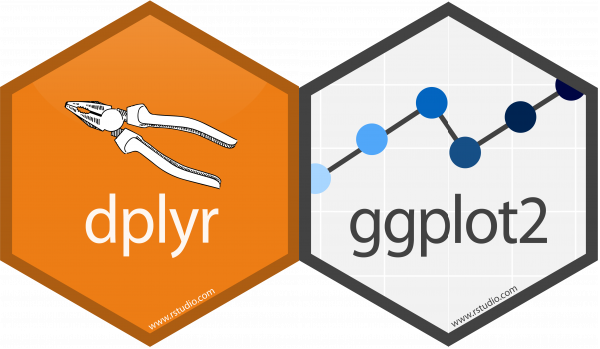
\includegraphics[scale=0.2]{slides_files/figure-beamer/dplyrggplot2.png}
\end{figure}

\end{frame}

\begin{frame}{What is GitHub?}
\protect\hypertarget{what-is-github}{}

\begin{itemize}
\tightlist
\item
  Website that hosts software development and version control using Git
\item
  Free basic services
\item
  Truly open source
\item
  ``Facebook for programmers''
\end{itemize}

\begin{figure}
  
\includegraphics[scale=0.2]{slides_files/figure-beamer/GitHub.png}
\end{figure}

\end{frame}

\begin{frame}{Why write R package?}
\protect\hypertarget{why-write-r-package}{}

\begin{itemize}
\tightlist
\item
  For yourself

  \begin{itemize}
  \tightlist
  \item
    Save time

    \begin{itemize}
    \tightlist
    \item
      Keep track of your functions
    \item
      Have all your functions in one place
    \end{itemize}
  \item
    Document your work
  \item
    For publishing papers

    \begin{itemize}
    \tightlist
    \item
      Increasingly, (bio)statistical journals ask for R package
      development of novel method
    \end{itemize}
  \end{itemize}
\item
  For others

  \begin{itemize}
  \tightlist
  \item
    If package is useful to you, it is also useful to someone else
  \item
    Readers of your paper can use proposed method
  \item
    Advance science!
  \end{itemize}
\end{itemize}

\end{frame}

\begin{frame}{Why publish package on GitHub?}
\protect\hypertarget{why-publish-package-on-github}{}

\begin{itemize}
\tightlist
\item
  Reproducibility
\item
  Accessibility
\item
  Collaboration
\item
  Back-up method
\item
  Version-control using \alert{git} (more on this later)
\end{itemize}

\end{frame}

\begin{frame}[fragile]{What do you need to write R package?}
\protect\hypertarget{what-do-you-need-to-write-r-package}{}

\begin{itemize}
\tightlist
\item
  R Studio (\url{https://rstudio.com/})
\item
  \texttt{devtools} \& \texttt{roxygen2} packages
\item
  Git (install from \url{https://git-scm.com/})
\item
  GitHub account (\url{https://github.com/})
\end{itemize}

\textcolor{blue}{Some other useful packages}

\begin{itemize}
\tightlist
\item
  \texttt{here}
\item
  \texttt{available}
\end{itemize}

\begin{figure}
  \includegraphics[scale=0.2]{slides_files/figure-beamer/Rstudio.png}
\end{figure}

\end{frame}

\begin{frame}[fragile]{Let's begin!}
\protect\hypertarget{lets-begin}{}

\textbf{Major steps}

\small

\begin{enumerate}
\tightlist
\item
  Open R Studio

  \begin{enumerate}
  [i)]
  \tightlist
  \item
    New Project \(\rightarrow\) New Directory \(\rightarrow\) R Package
    \(\rightarrow\) Enter info \(\rightarrow\) Create Project
  \end{enumerate}
\item
  Write functions

  \begin{enumerate}
  [i)]
  \tightlist
  \item
    Each function should be saved in its own file
  \item
    Write package description and document functions
  \end{enumerate}
\item
  Create new repo in GitHub

  \begin{enumerate}
  [i)]
  \tightlist
  \item
    Repo name \(=\) package name
  \end{enumerate}
\item
  Connect to GitHub
\item
  Pull + Commit + Push
\item
  Use/share package with \texttt{install\_github()}!
\end{enumerate}

\centering

\alert{There is more than one way!}

\end{frame}

\begin{frame}[fragile]{Naming R package}
\protect\hypertarget{naming-r-package}{}

Some tips:

\begin{itemize}
\tightlist
\item
  Make it simple \& short
\item
  Make it unique (use \texttt{available} package -- see next slide)
\item
  Must start with a letter \& cannot end with a period
\item
  Do not use special characters
\item
  Trend towards using all lower case
\item
  Hadley's book has
  \href{https://r-pkgs.org/workflows101.html?q=naming\#naming}{more
  information}
\end{itemize}

\end{frame}

\begin{frame}[fragile]{Naming R package}
\protect\hypertarget{naming-r-package-1}{}

Check to see if name is unique, especially if you plan to submit to CRAN
\footnotesize

\begin{Shaded}
\begin{Highlighting}[]
\KeywordTok{install.packages}\NormalTok{(}\StringTok{"available"}\NormalTok{)}
\KeywordTok{library}\NormalTok{(available)}
\end{Highlighting}
\end{Shaded}

\begin{Shaded}
\begin{Highlighting}[]
\CommentTok{#available("ayapack", browse = FALSE)}
\end{Highlighting}
\end{Shaded}

\end{frame}

\begin{frame}{In RStudio}
\protect\hypertarget{in-rstudio}{}

\begin{itemize}
\tightlist
\item
  New Project \(\rightarrow\) New Directory \(\rightarrow\) R Package

  \begin{itemize}
  \tightlist
  \item
    Enter package name
  \item
    Optional: Select R scripts that include your functions (if you leave
    blank, a default function is included)
  \item
    Select subdirectory where you want to save the package (location is
    not too important since the final product will be saved on Github)
  \item
    Check \alert{`Create a git repository`}
  \end{itemize}
\end{itemize}

\begin{figure}
  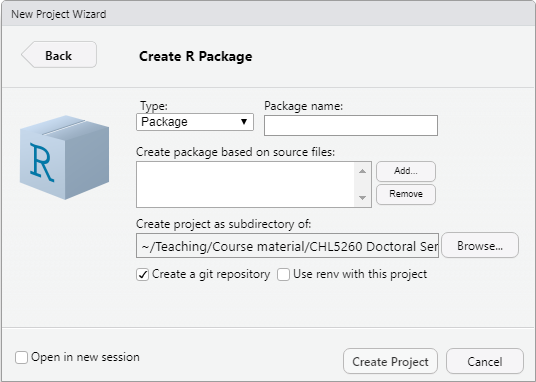
\includegraphics[scale=0.4]{slides_files/figure-beamer/Rstudio_packagesetup.png}
\end{figure}

\end{frame}

\begin{frame}[fragile]{In RStudio}
\protect\hypertarget{in-rstudio-1}{}

This will create the following files and folders

\small

\begin{itemize}
\tightlist
\item
  \alert{packagename.Rproj}: This indicates that the directory is a
  project
\item
  \alert{DESCRIPTION}: This is where all the meta-data about your
  package goes -- you can edit this file manually
\item
  \alert{NAMESPACE}: This file indicates what needs to be exposed to
  users for your R package -- we will recreate this file using
  \texttt{document()} (see next slide)
\item
  \alert{R}: This is where all your R code goes for your package
\item
  \alert{man}: This is where the manuals for your functions will be
  saved
\item
  Don't worry too much about the rest (.gitignore, .Rbuildingore)
\end{itemize}

\begin{figure}
  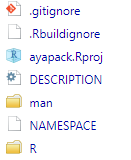
\includegraphics[scale=0.55]{slides_files/figure-beamer/package1.png}
\end{figure}

\end{frame}

\begin{frame}[fragile]{In RStudio}
\protect\hypertarget{in-rstudio-2}{}

Next, load the \texttt{devtools} package

\begin{Shaded}
\begin{Highlighting}[]
\KeywordTok{library}\NormalTok{(devtools)}
\end{Highlighting}
\end{Shaded}

Then, delete the NAMESPACE file

\end{frame}

\begin{frame}{Great resources}
\protect\hypertarget{great-resources}{}

\begin{itemize}
\tightlist
\item
  \href{https://r-pkgs.org/}{Book by Hadley Wickham and Jenny Bryan}
\item
  \href{https://rstudio.com/wp-content/uploads/2015/03/devtools-cheatsheet.pdf}{devtools
  cheatsheet}
\item
  \href{https://www.mzes.uni-mannheim.de/socialsciencedatalab/article/r-package/}{Blog
  post by MZES Social Science Data La}
\end{itemize}

\end{frame}

\begin{frame}[fragile]{Turn this project into a package}
\protect\hypertarget{turn-this-project-into-a-package}{}

\begin{Shaded}
\begin{Highlighting}[]
\NormalTok{devtools}\OperatorTok{::}\KeywordTok{create}\NormalTok{(here}\OperatorTok{::}\KeywordTok{here}\NormalTok{())}
\end{Highlighting}
\end{Shaded}

This will create 3 additional files

\begin{itemize}
\tightlist
\item
  DESCRIPTION: This is where all the meta-data about your package goes.
  You can edit this file manually.
\item
  NAMESPACE: This file indicates what needs to be exposed to users for
  your R package. Do not edit this file.
\item
  R: This is where all your R code goes for your package.
\end{itemize}

\end{frame}

\begin{frame}[fragile]{Add your function}
\protect\hypertarget{add-your-function}{}

Open new R script and write your function

\begin{Shaded}
\begin{Highlighting}[]
\NormalTok{myfunc <-}\StringTok{ }\ControlFlowTok{function}\NormalTok{(x)\{}
\NormalTok{  y <-}\StringTok{ }\NormalTok{x }\OperatorTok{+}\StringTok{ }\NormalTok{x}
  \KeywordTok{return}\NormalTok{(y)}
\NormalTok{\}}
\end{Highlighting}
\end{Shaded}

\end{frame}

\begin{frame}[fragile]{Add your function}
\protect\hypertarget{add-your-function-1}{}

Include \texttt{@export} tag above your function to indicate this
function to be ``exposed'' to users.

\begin{Shaded}
\begin{Highlighting}[]
\CommentTok{#' @export}
\NormalTok{myfunc <-}\StringTok{ }\ControlFlowTok{function}\NormalTok{(x)\{}
\NormalTok{  y <-}\StringTok{ }\NormalTok{x }\OperatorTok{+}\StringTok{ }\NormalTok{x}
  \KeywordTok{return}\NormalTok{(y)}
\NormalTok{\}}
\end{Highlighting}
\end{Shaded}

\end{frame}

\begin{frame}[fragile]{Add your function}
\protect\hypertarget{add-your-function-2}{}

Also, include documentation for your function when you go
\texttt{?myfunc}. \small

\begin{Shaded}
\begin{Highlighting}[]
\CommentTok{#' This is my function.}
\CommentTok{#'}
\CommentTok{#' This function returns a value from adding the parameters.}
\CommentTok{#' @param x}
\CommentTok{#' @return y}
\CommentTok{#' @export}
\NormalTok{myfunc <-}\StringTok{ }\ControlFlowTok{function}\NormalTok{(x)\{}
\NormalTok{  y <-}\StringTok{ }\NormalTok{x }\OperatorTok{+}\StringTok{ }\NormalTok{x}
  \KeywordTok{return}\NormalTok{(y)}
\NormalTok{\}}
\end{Highlighting}
\end{Shaded}

\end{frame}

\begin{frame}[fragile]{Add your function}
\protect\hypertarget{add-your-function-3}{}

Now run

\begin{Shaded}
\begin{Highlighting}[]
\NormalTok{devtools}\OperatorTok{::}\KeywordTok{document}\NormalTok{()}
\end{Highlighting}
\end{Shaded}

\begin{itemize}
\tightlist
\item
  This will create \texttt{man} directory that includes read-only file
  \texttt{myfunc.Rd}
\item
  Note that \texttt{NAMESPACE} file has been updated
\end{itemize}

\end{frame}

\begin{frame}{Add data set}
\protect\hypertarget{add-data-set}{}

\end{frame}

\begin{frame}{In GitHub}
\protect\hypertarget{in-github}{}

First, log in and go to Repositories

\begin{figure}
  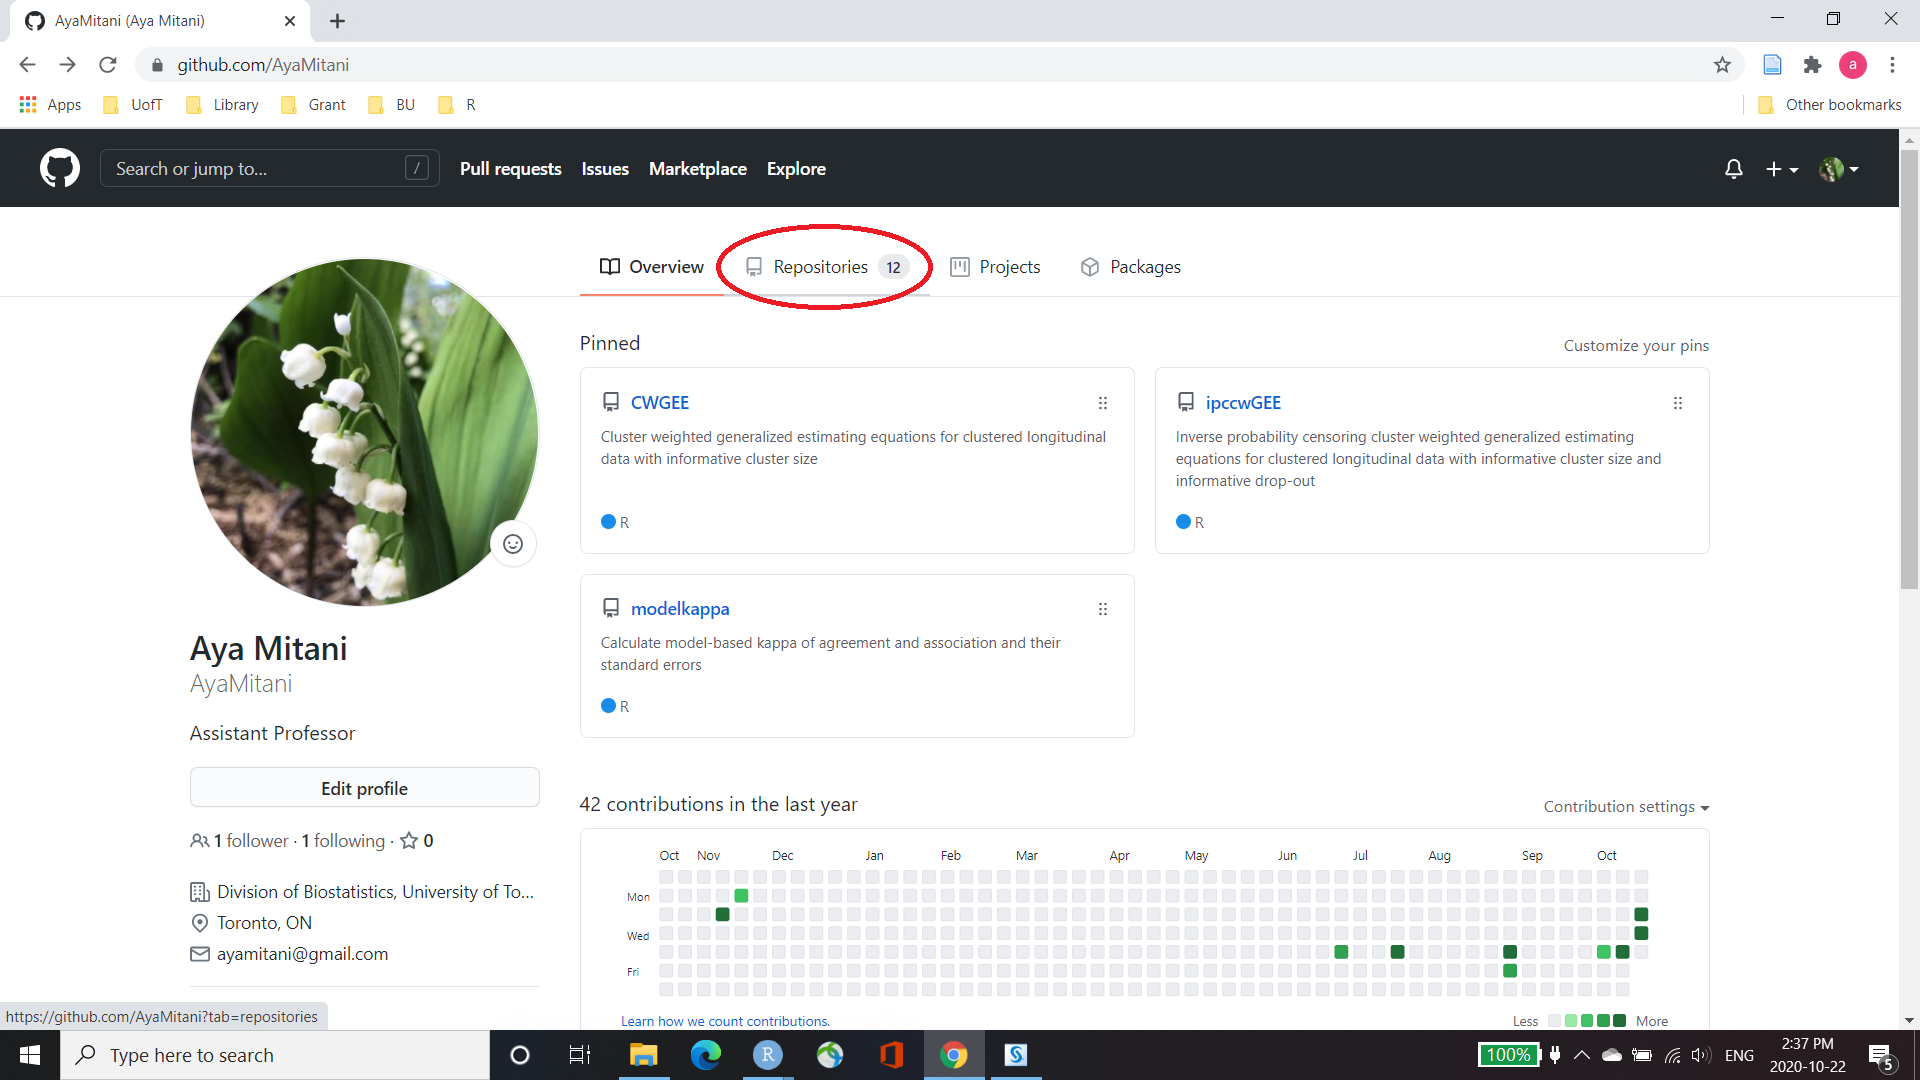
\includegraphics[scale=0.275]{slides_files/figure-beamer/GitHub_step1.png}
\end{figure}

\end{frame}

\begin{frame}{In GitHub}
\protect\hypertarget{in-github-1}{}

Then, create new repository

\begin{figure}
  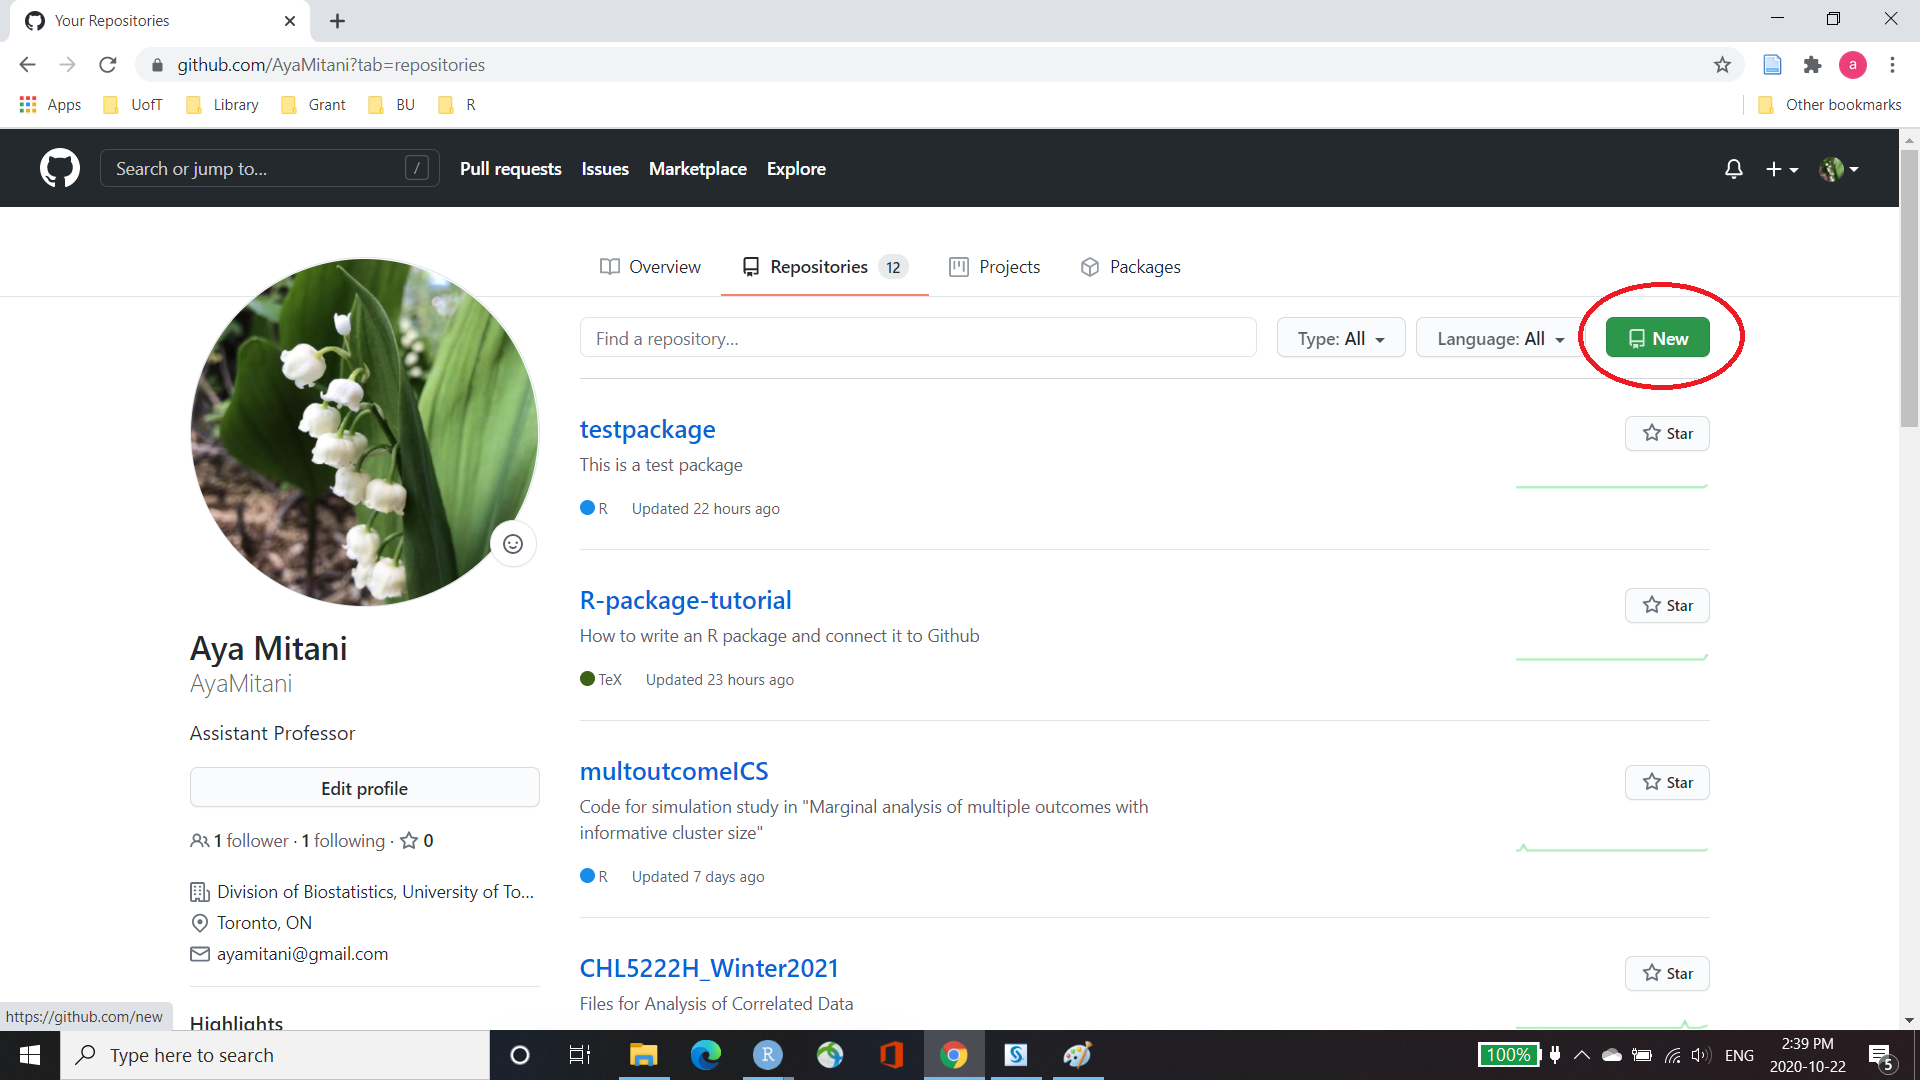
\includegraphics[scale=0.275]{slides_files/figure-beamer/GitHub_step2.png}
\end{figure}

\end{frame}

\begin{frame}{In GitHub}
\protect\hypertarget{in-github-2}{}

Repo name should be same as package name

\begin{figure}
  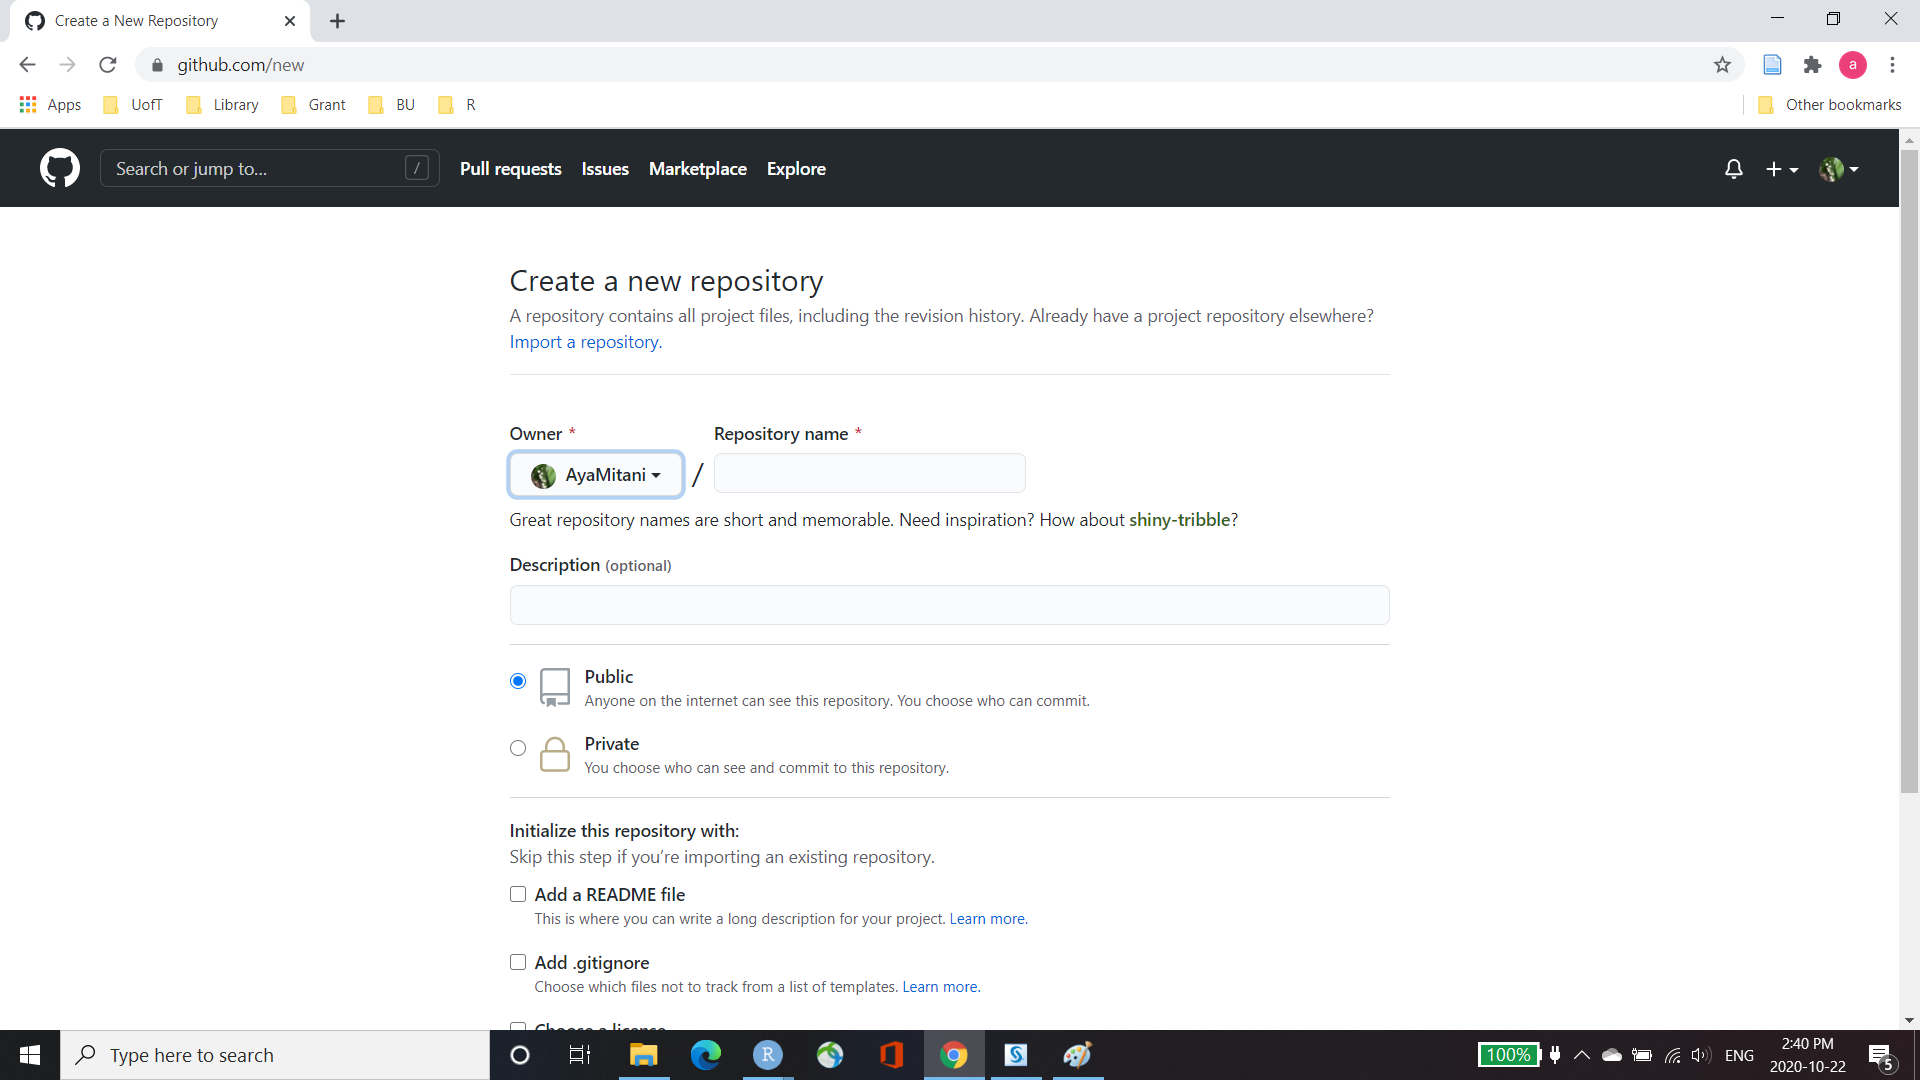
\includegraphics[scale=0.275]{slides_files/figure-beamer/GitHub_step3.png}
\end{figure}

\end{frame}

\begin{frame}{In GitHub}
\protect\hypertarget{in-github-3}{}

Finish creating new repo

\begin{figure}
  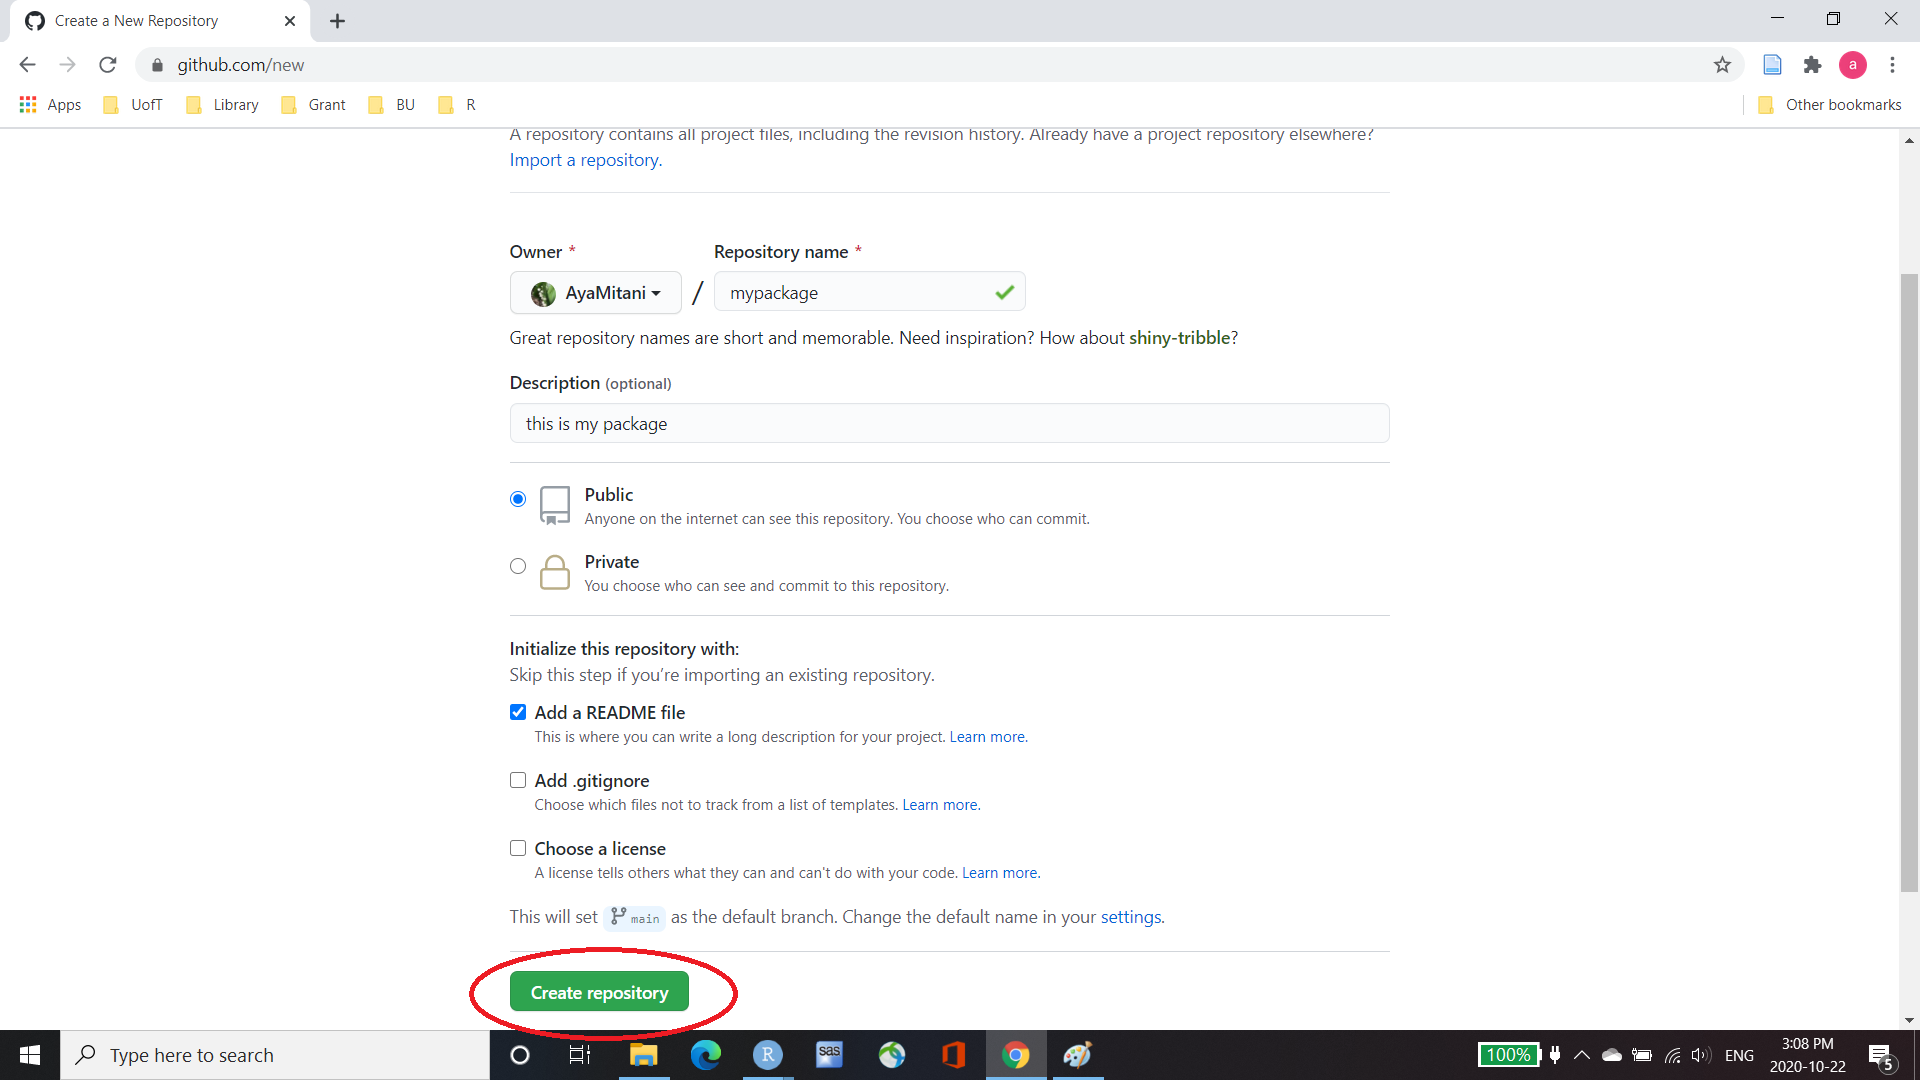
\includegraphics[scale=0.275]{slides_files/figure-beamer/GitHub_step4.png}
\end{figure}

\end{frame}

\begin{frame}{In GitHub}
\protect\hypertarget{in-github-4}{}

Finally, copy URL

\begin{figure}
  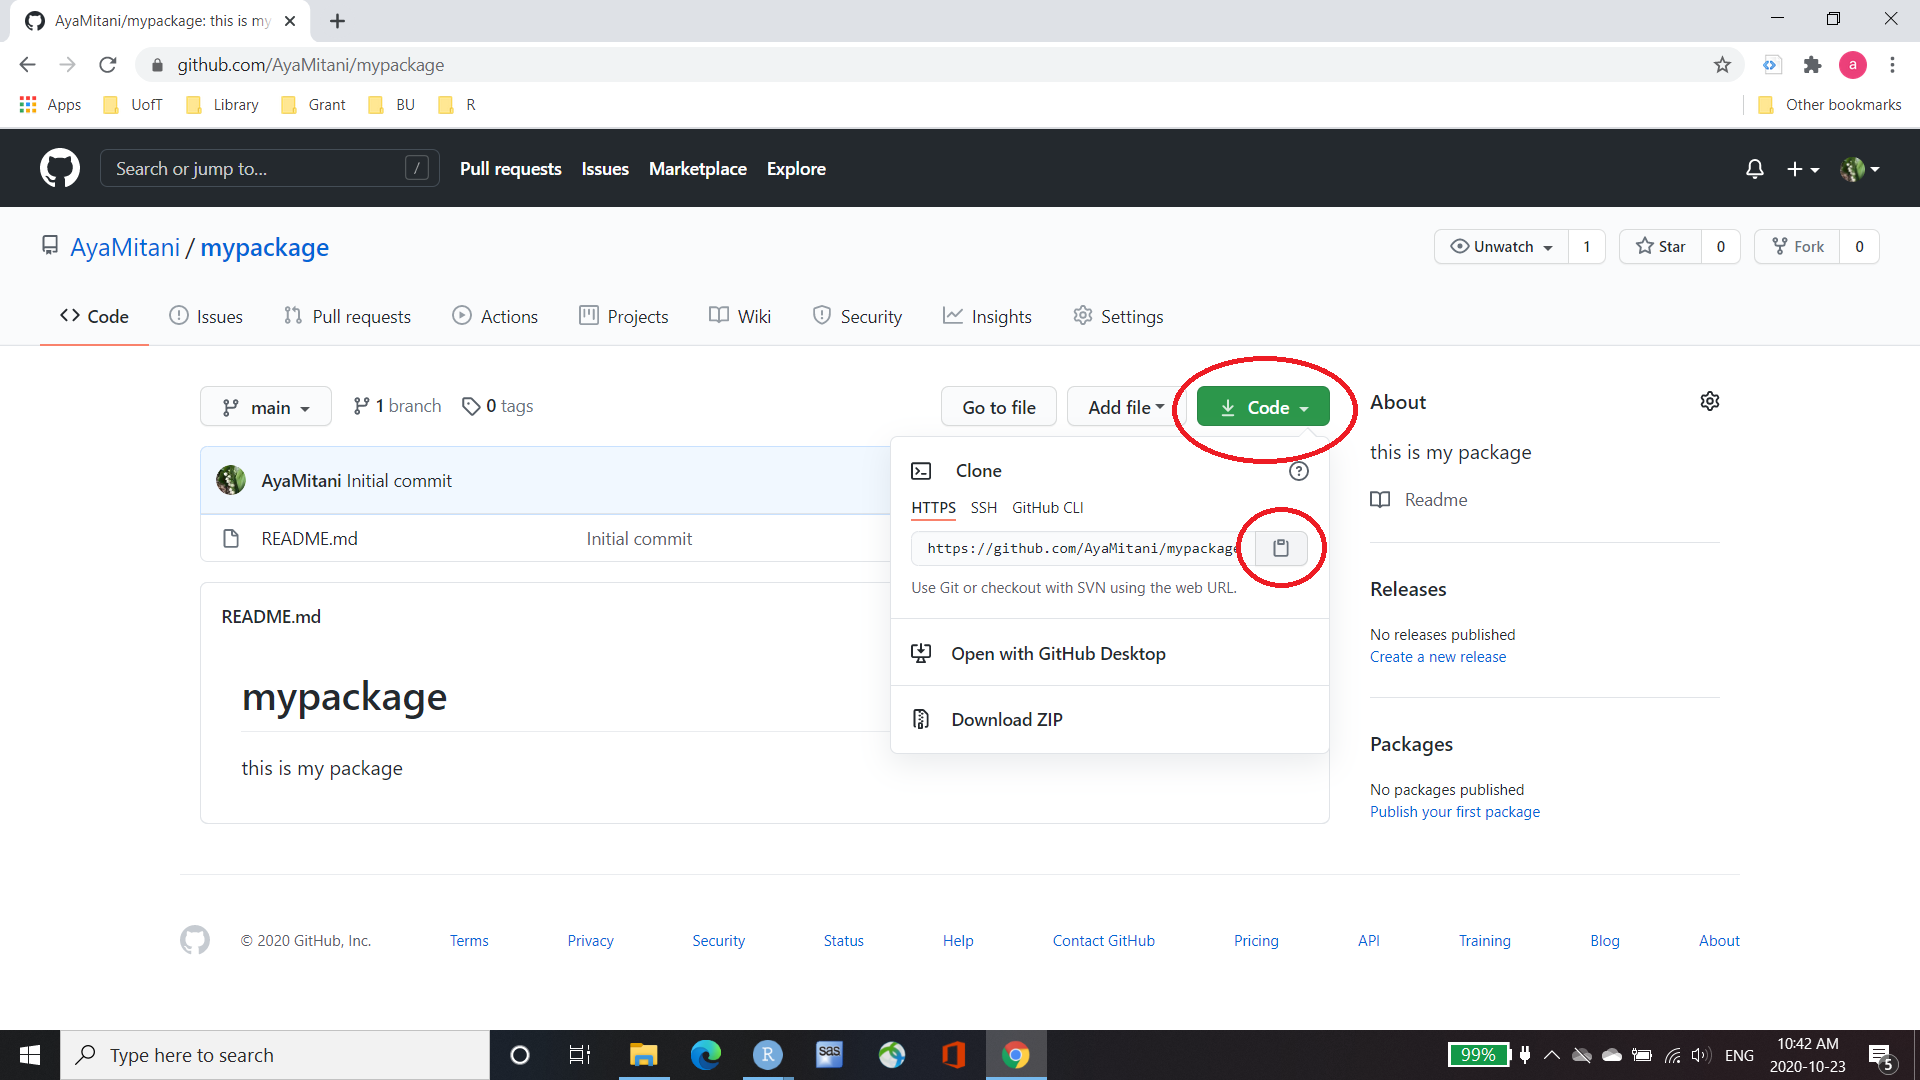
\includegraphics[scale=0.275]{slides_files/figure-beamer/GitHub_step5.png}
\end{figure}

\end{frame}

\end{document}
